\documentclass[11pt]{beamer}
% \usetheme{Boadilla}
  \usetheme{default}


% acronyms for text or math mode
\newcommand {\ccast} {\mbox{\small CCAST}}
\newcommand {\cris} {\mbox{\small CrIS}}

\newcommand {\airs} {\mbox{\small AIRS}}
\newcommand {\iasi} {\mbox{\small IASI}}
\newcommand {\idps} {\mbox{\small IDPS}}
\newcommand {\nasa} {\mbox{\small NASA}}
\newcommand {\noaa} {\mbox{\small NOAA}}
\newcommand {\nstar} {\mbox{\small STAR}}
\newcommand {\umbc} {\mbox{\small UMBC}}
\newcommand {\uw}   {\mbox{\small UW}}

\newcommand {\fft}  {\mbox{\small FFT}}
\newcommand {\ifft} {\mbox{\small IFFT}}
\newcommand {\fir}  {\mbox{\small FIR}}
\newcommand {\fov}  {\mbox{\small FOV}}
\newcommand {\for}  {\mbox{\small FOR}}
\newcommand {\ict}  {\mbox{\small ICT}}
\newcommand {\ils}  {\mbox{\small ILS}}
\newcommand {\igm}  {\mbox{\small IGM}}
\newcommand {\opd}  {\mbox{\small OPD}}
\newcommand {\rms}  {\mbox{\small RMS}}
\newcommand {\zpd}  {\mbox{\small ZPD}}
\newcommand {\ppm}  {\mbox{\small PPM}}
\newcommand {\srf}  {\mbox{\small SRF}}
\newcommand {\sdr}  {\mbox{\small SDR}}

\newcommand {\ES} {\mbox{\small ES}}
\newcommand {\SP} {\mbox{\small SP}}
\newcommand {\IT} {\mbox{\small IT}}
\newcommand {\SA} {\mbox{\small SA}}

\newcommand {\ET} {\mbox{\small ET}}
\newcommand {\FT} {\mbox{\small FT}}

% abbreviations, mainly for math mode
\newcommand {\real} {\mbox{real}}
\newcommand {\imag} {\mbox{imag}}
\newcommand {\atan} {\mbox{atan}}
\newcommand {\obs}  {\mbox{obs}}
\newcommand {\calc} {\mbox{calc}}
\newcommand {\sinc} {\mbox{sinc}}
\newcommand {\psinc} {\mbox{psinc}}
\newcommand {\std} {\mbox{std}}

% symbols, for math mode only
\newcommand {\wnum} {\mbox{cm$^{-1}$}}
\newcommand {\lmax} {L_{\mbox{\tiny max}}}
\newcommand {\vmax} {V_{\mbox{\tiny max}}}

\newcommand {\tauobs} {\tau_{\mbox{\tiny obs}}}
\newcommand {\taucal} {\tau_{\mbox{\tiny calc}}}
\newcommand {\Vdc}  {V_{\mbox{\tiny DC}}}

\newcommand {\rIT} {r_{\mbox{\tiny\textsc{ict}}}}
\newcommand {\rES} {r_{\mbox{\tiny\textsc{es}}}}
\newcommand {\robs} {r_{\mbox{\tiny obs}}}

\newcommand {\rITobs} {r_{\mbox{\tiny\textsc{ict}}}^{\mbox{\tiny obs}}}
\newcommand {\rITcal} {r_{\mbox{\tiny\textsc{ict}}}^{\mbox{\tiny cal}}}

\newcommand {\ITmean} {\langle\mbox{\small IT}\rangle}
\newcommand {\SPmean} {\langle\mbox{\small SP}\rangle}


\title{cris extended resolution \\
       calibration algorithm comparisons \\
\vspace{4mm}
{****} DRAFT {****} \\
}
\author{H.~E.~Motteler, L.~L.~Strow}
\institute{
  UMBC Atmospheric Spectroscopy Lab \\
  Joint Center for Earth Systems Technology \\
}
\date{\today}
\begin{document}

%----------- slide --------------------------------------------------%
\begin{frame}[plain]
\titlepage
\end{frame}
%----------- slide --------------------------------------------------%
\begin{frame}
\frametitle{introduction}

\begin{itemize}

  \item we compare the {\umbc} {\ccast} implementations of our
    reference and the \noaa~4 calibration algorithms on extended
    resolution data

  \item this allows for identical \ils\ and processing details---the
    only difference in tests is the form of the calibration equation

  \item we show results for both clear matchups and \fov~5 relative
    tests.  For matchups we compare the {\ccast} algorithm with flat
    reference truth and \noaa~4 with reference truth convolved with
    instrument responsivity

\end{itemize}

\end{frame}
%----------- slide --------------------------------------------------%
\begin{frame}
\frametitle{methods}

\begin{itemize}

  \item for tests with calculated radiance we start with 3782 clear
    matchups from ccast granule SDR\_d20160120\_t0304487 and
    calculate upwelling radiances with kcarta at a 0.0025 cm-1 grid

  \item for the ``flat'' tests the ccast processing filters are
    applied pointwise and the result is convolved to the {\cris}
    user grid

  \item for the ``resp'' tests instrument responsivity is applied
    pointwise to the kcarta radiances, these are convolved to the
    user grid, and then divided pointwise by inverse responsivity

  \item relative tests are with data averaged over the three day
    test period, 18-20 Jan 2016
    
  \item all test are done with periodic sinc wrapping at the sensor
    grid, cosine apodization of the extended res points, the old a2
    weights, and double Fourier interpolation to the user grid

\end{itemize}

\end{frame}
%----------- slide --------------------------------------------------%
\begin{frame}
\frametitle{obs minus calc overview}
\begin{center}
  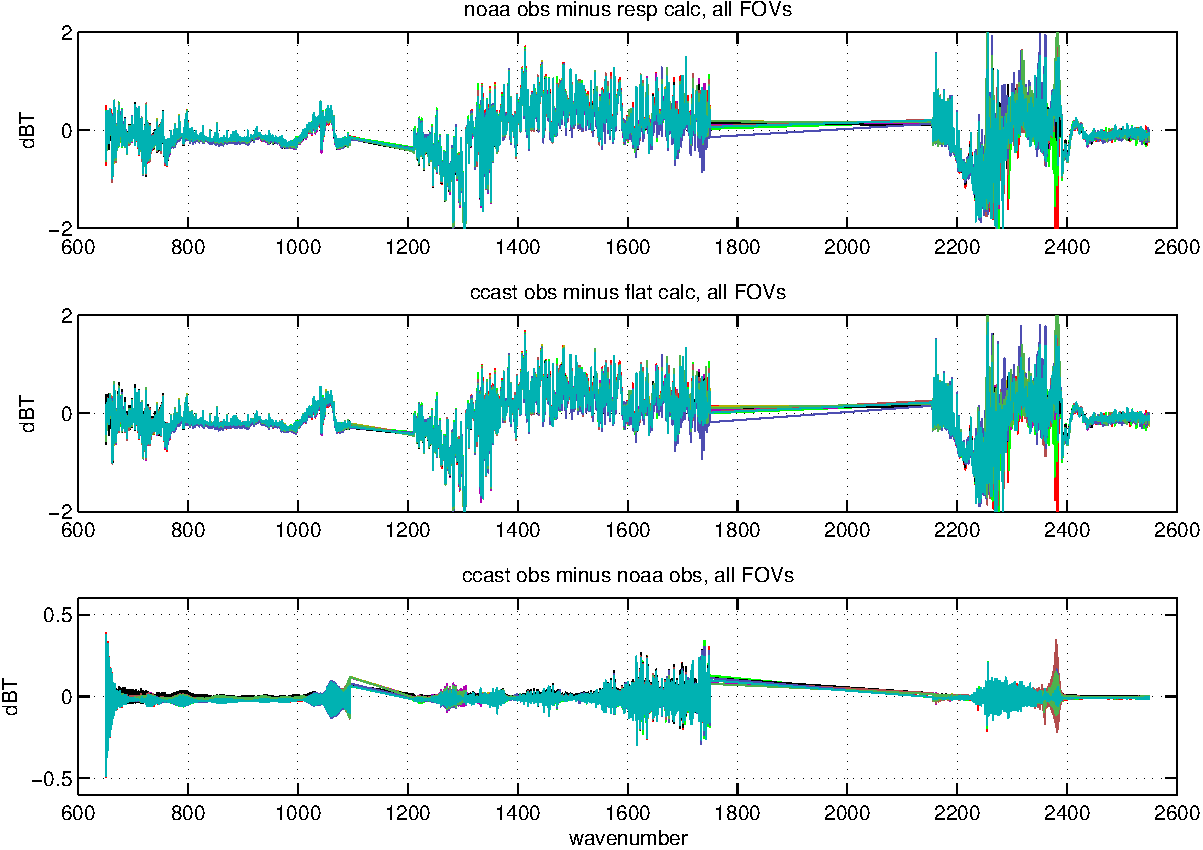
\includegraphics[scale=0.5]{figures/cal_summary.pdf}
\end{center}
\end{frame}
%----------- slide --------------------------------------------------%
\begin{frame}
\frametitle{obs minus calc LW detail}
\begin{center}
  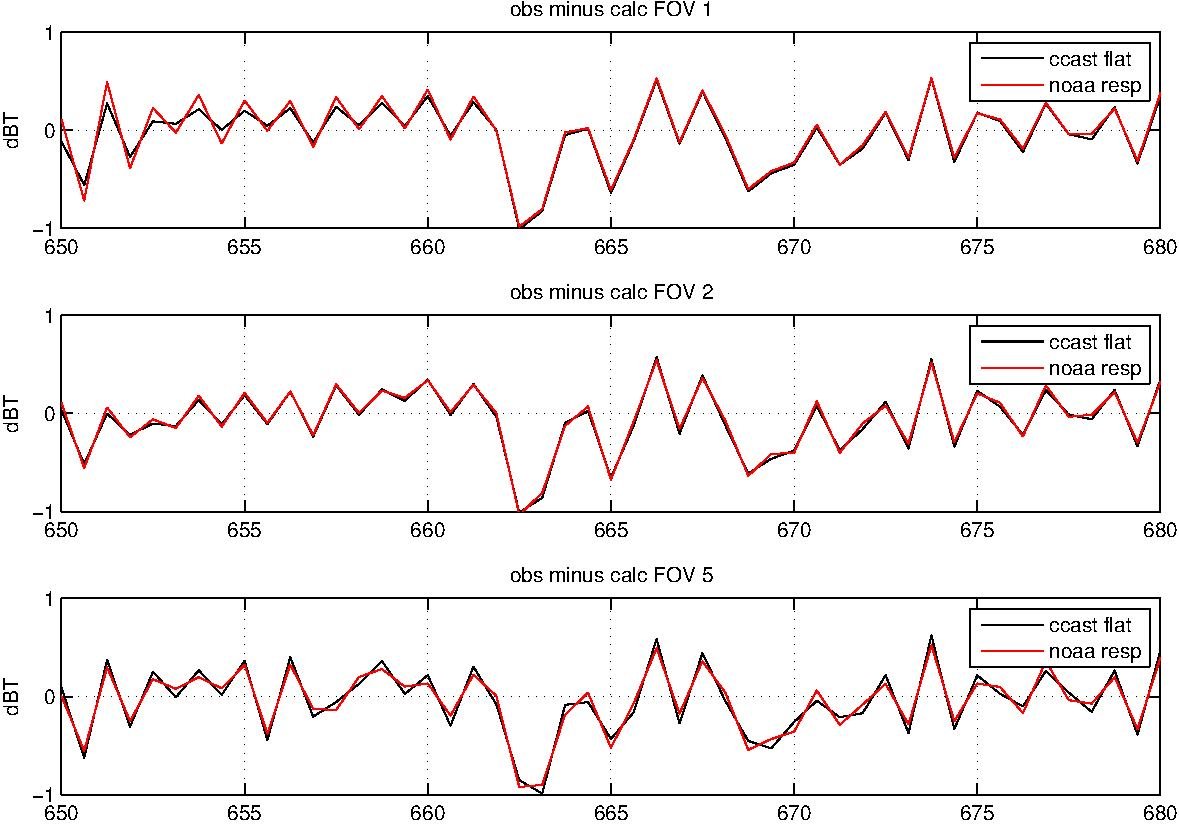
\includegraphics[scale=0.5]{figures/cal_LW_detail.pdf}
\end{center}
\end{frame}
%----------- slide --------------------------------------------------%
\begin{frame}
\frametitle{noaa all fovs LW detail}
\begin{center}
  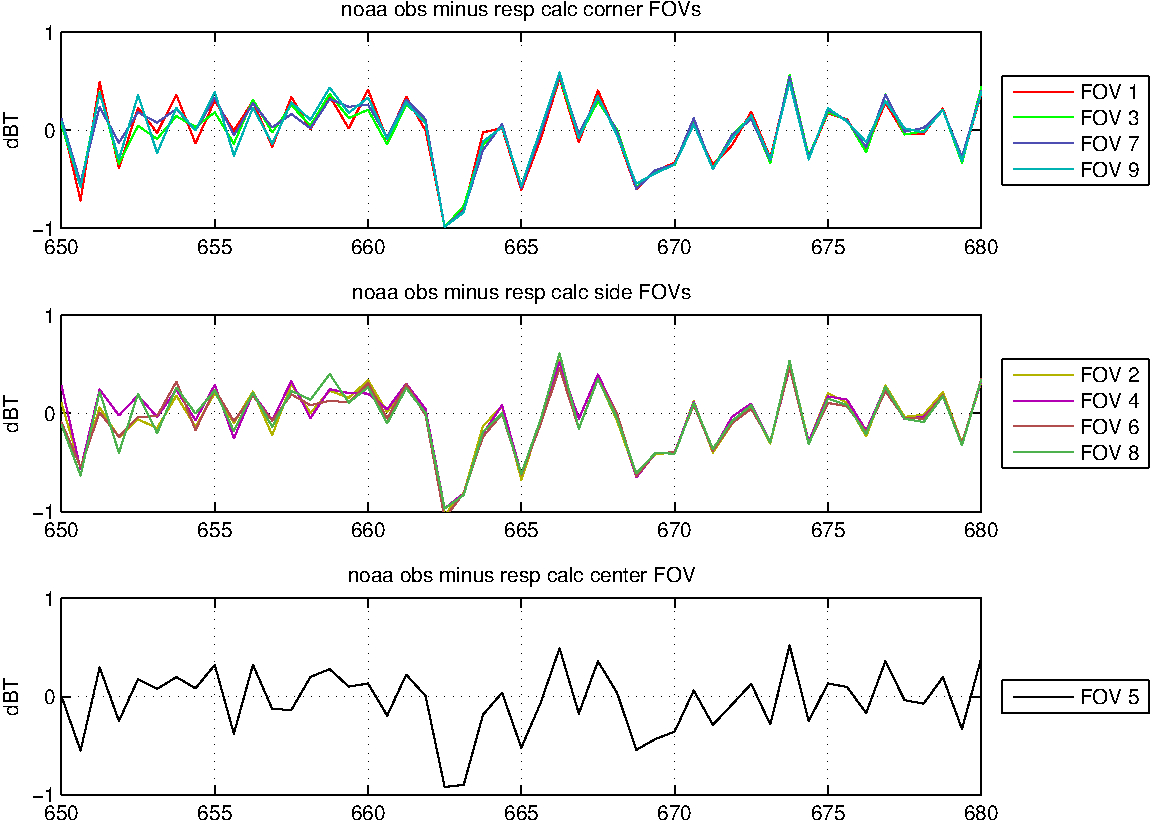
\includegraphics[scale=0.5]{figures/cal_noaa_LW.pdf}
\end{center}
\end{frame}
%----------- slide --------------------------------------------------%
\begin{frame}
\frametitle{ccast all fovs LW detail}
\begin{center}
  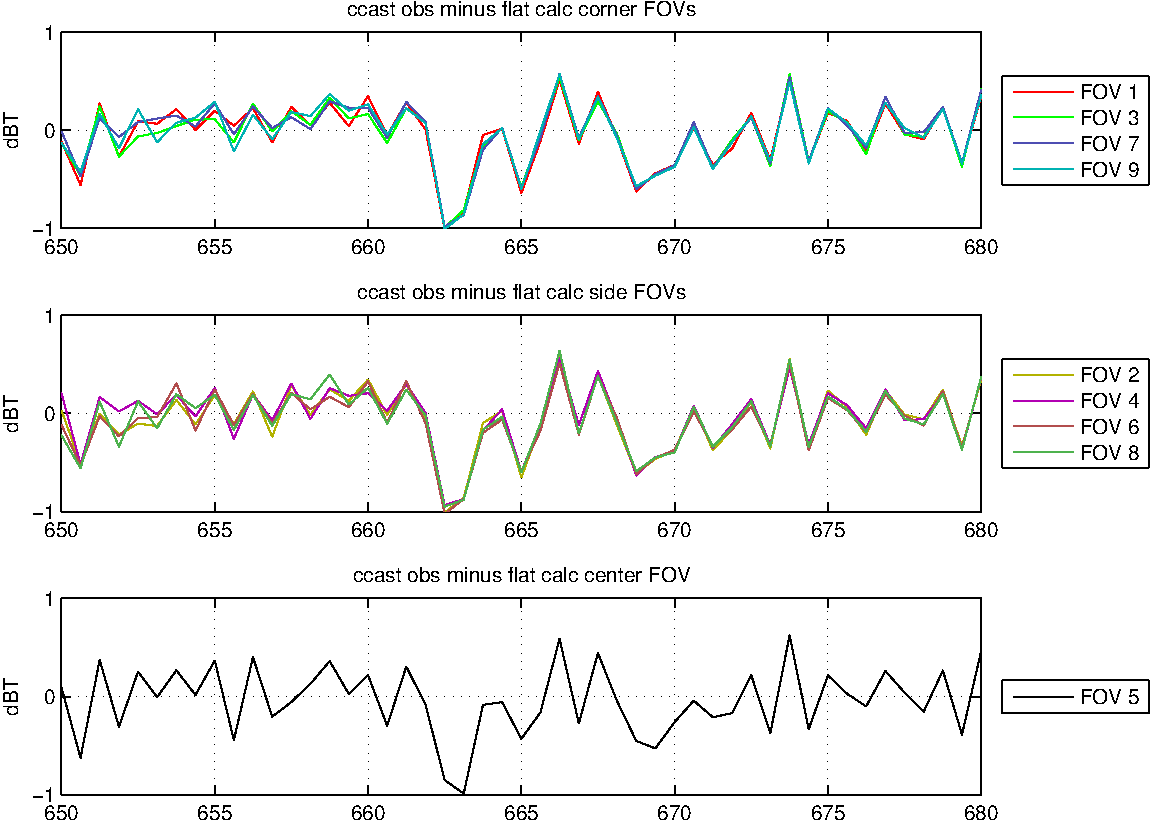
\includegraphics[scale=0.5]{figures/cal_ccast_LW.pdf}
\end{center}
\end{frame}
%----------- slide --------------------------------------------------%
\begin{frame}
\frametitle{obs minus calc MW detail}
\begin{center}
  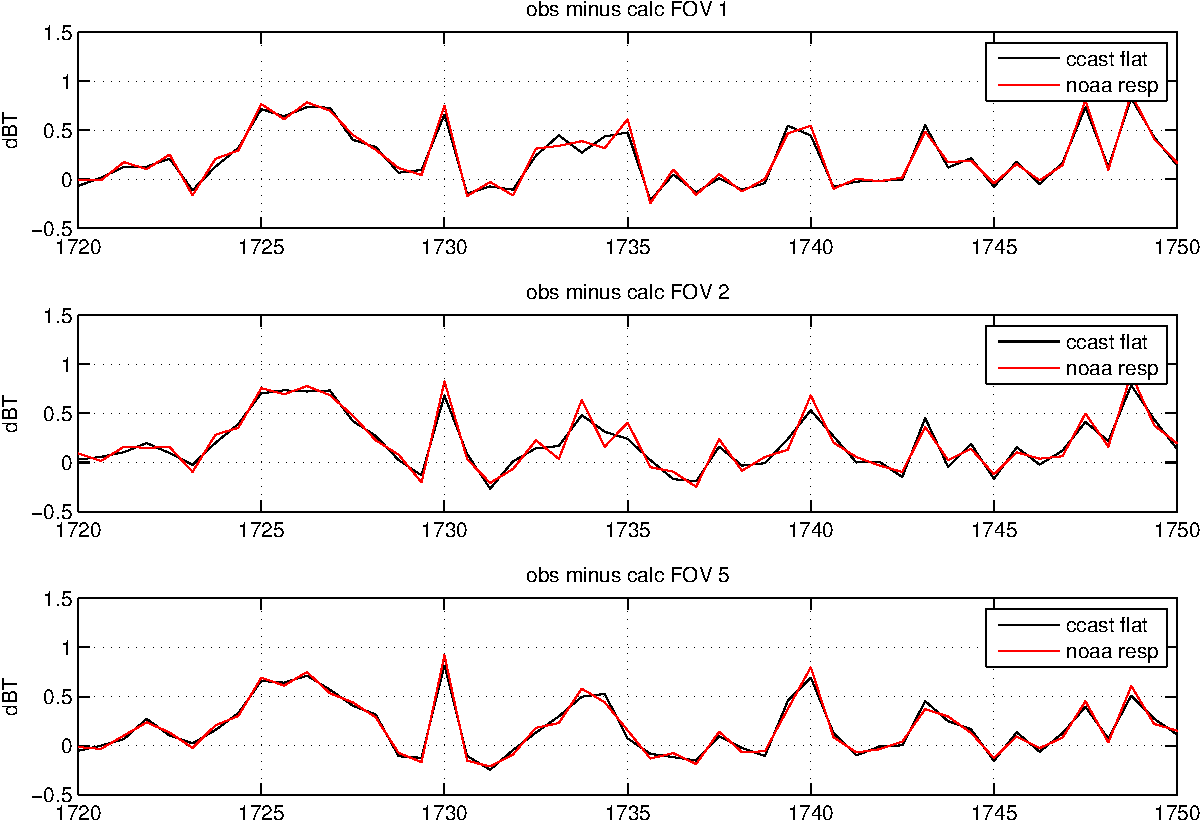
\includegraphics[scale=0.5]{figures/cal_MW_detail.pdf}
\end{center}
\end{frame}
%----------- slide --------------------------------------------------%
\begin{frame}
\frametitle{noaa all fovs MW detail}
\begin{center}
  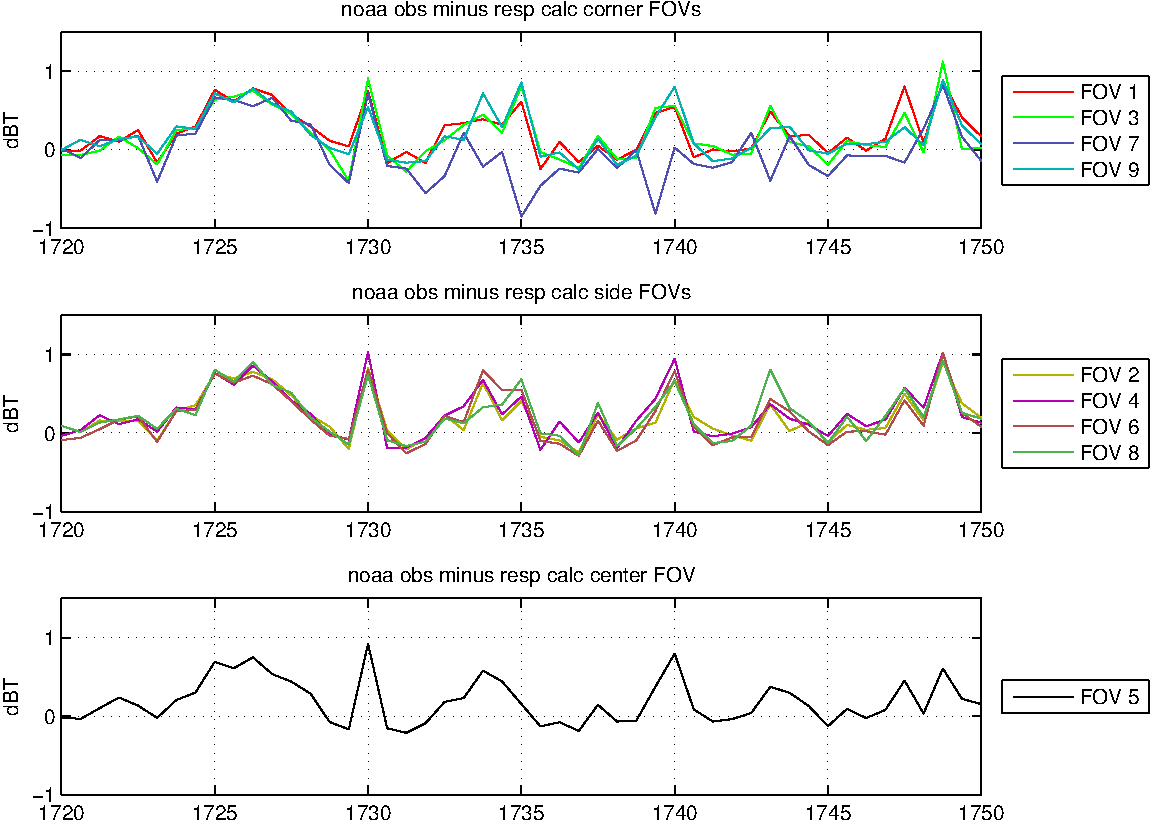
\includegraphics[scale=0.5]{figures/cal_noaa_MW.pdf}
\end{center}
\end{frame}
%----------- slide --------------------------------------------------%
\begin{frame}
\frametitle{ccast all fovs MW detail}
\begin{center}
  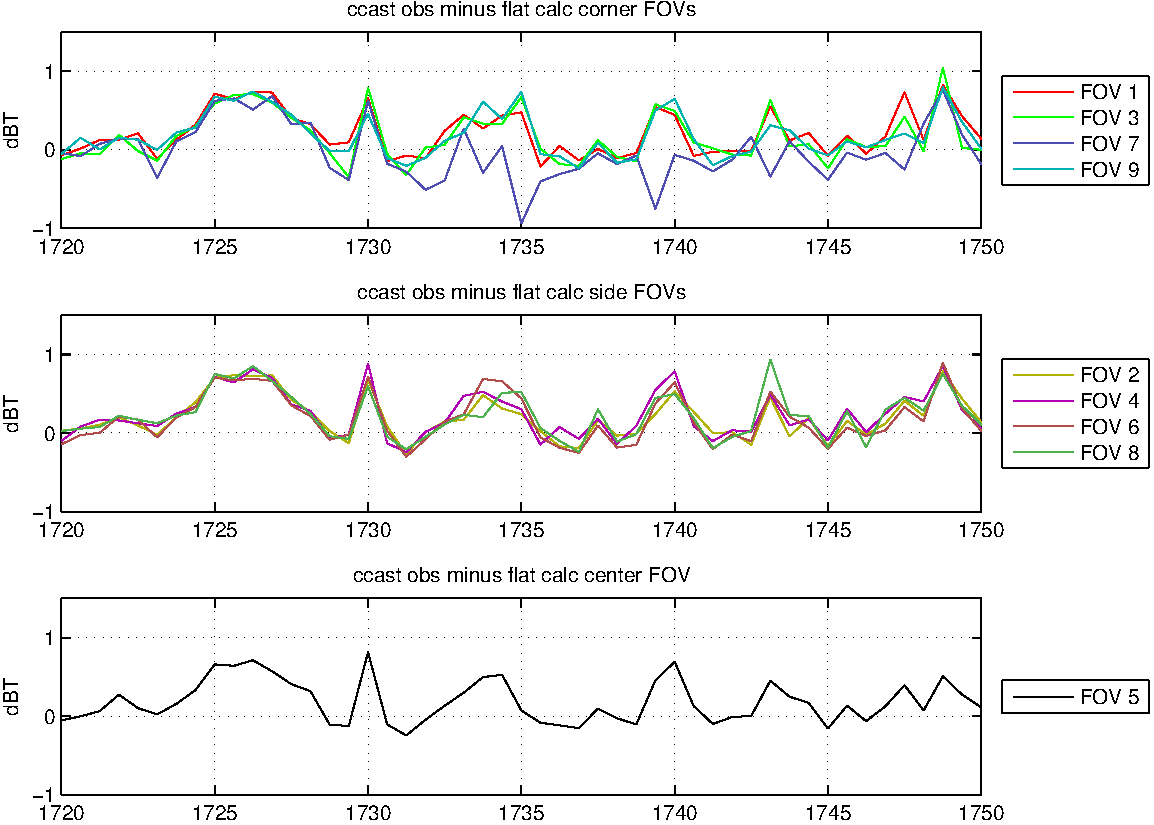
\includegraphics[scale=0.5]{figures/cal_ccast_MW.pdf}
\end{center}
\end{frame}
%----------- slide --------------------------------------------------%
\begin{frame}
\frametitle{obs minus calc summary}

\begin{itemize}

  \item {\ccast} minus flat and {\noaa} minus resp residuals are
    similar, significantly more so than for regular resolution
    processing

  \item the spectral intervals shown here here are regions where the
    differences between the algorithms was greatest for our 15 Aug
    2015 regular high resolution comparison

  \item below 680 \wn\ we see {\ccast} does slightly better for the
    side and corner FOVS, while {\noaa} is slightly better for FOV 5.  
    The {\ccast} residuals are more consistent across FOVs

  \item in the MW detail we see {\ccast} does slightly better for
    all FOVs.  These results are with the old a2 weights; the new
    UMBC a2 weights give a significant further reduction in the MW
    residuals

\end{itemize}

\end{frame}
%----------- slide --------------------------------------------------%
\begin{frame}
\frametitle{noaa resp and ccast flat double diffs}
\begin{center}
  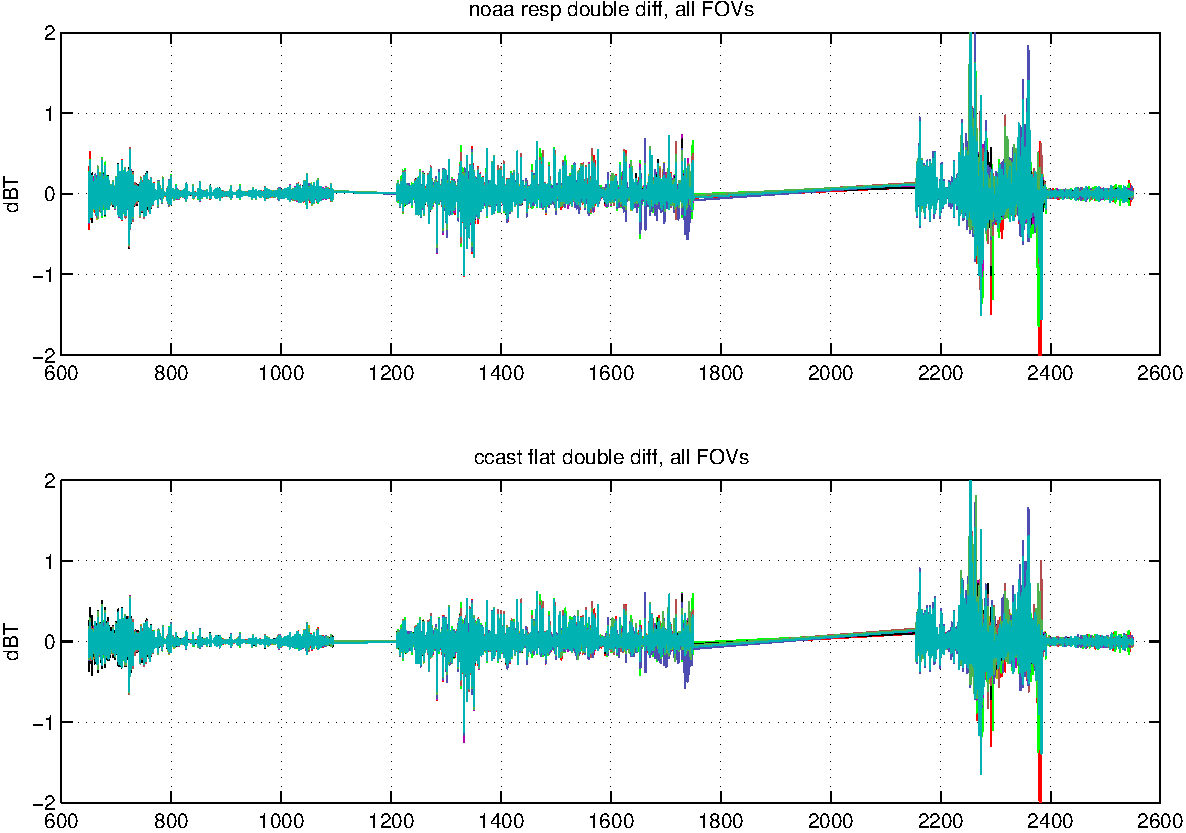
\includegraphics[scale=0.5]{figures/cal_ddif_1.pdf}
\end{center}
\end{frame}

%----------- slide --------------------------------------------------%
\begin{frame}
\frametitle{noaa flat and ccast resp double diffs}
\begin{center}
  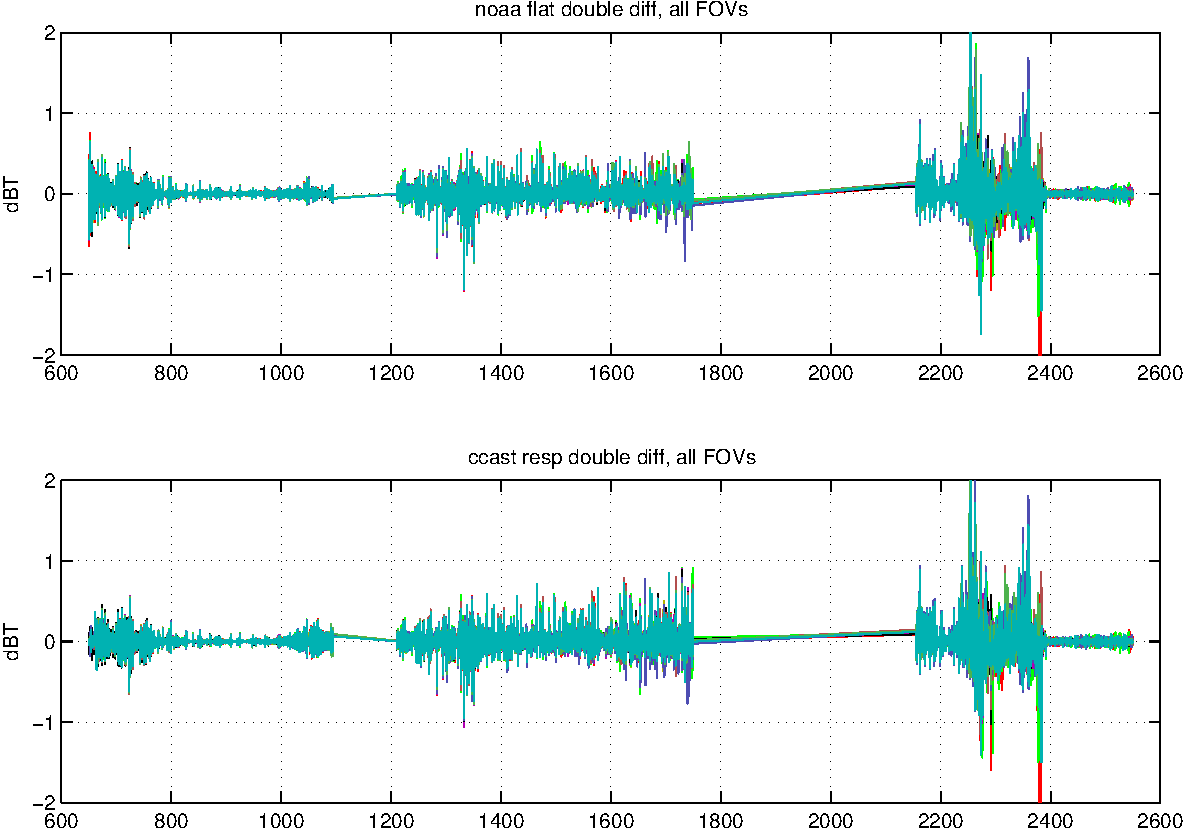
\includegraphics[scale=0.5]{figures/cal_ddif_2.pdf}
\end{center}
\end{frame}

%----------- slide --------------------------------------------------%
\begin{frame}
\frametitle{double difference summary}

\begin{itemize}

  \item the first double difference is 
    \[(\mbox{\small noaa obs} - \mbox{\small resp calc}) - 
       (\mbox{\small hamming noaa obs} - 
        \mbox{\small hamming resp calc})\]  

  \item the other double differences are analogous

  \item {\noaa} with responsivity and ccast with flat reference
    truth are similar, with {\ccast} slightly worse at the low end
    of the MW but slightly better in MW above around 1600 cm-1

  \item comparing {\noaa} with flat reference truth and {\ccast}
    with responsivity, we see both do slightly worse overall than
    when compared with their default reference truths.

\end{itemize}

\end{frame}

\end{document}

%----------- slide --------------------------------------------------%
\begin{frame}
\frametitle{relative test overview}
\begin{center}
  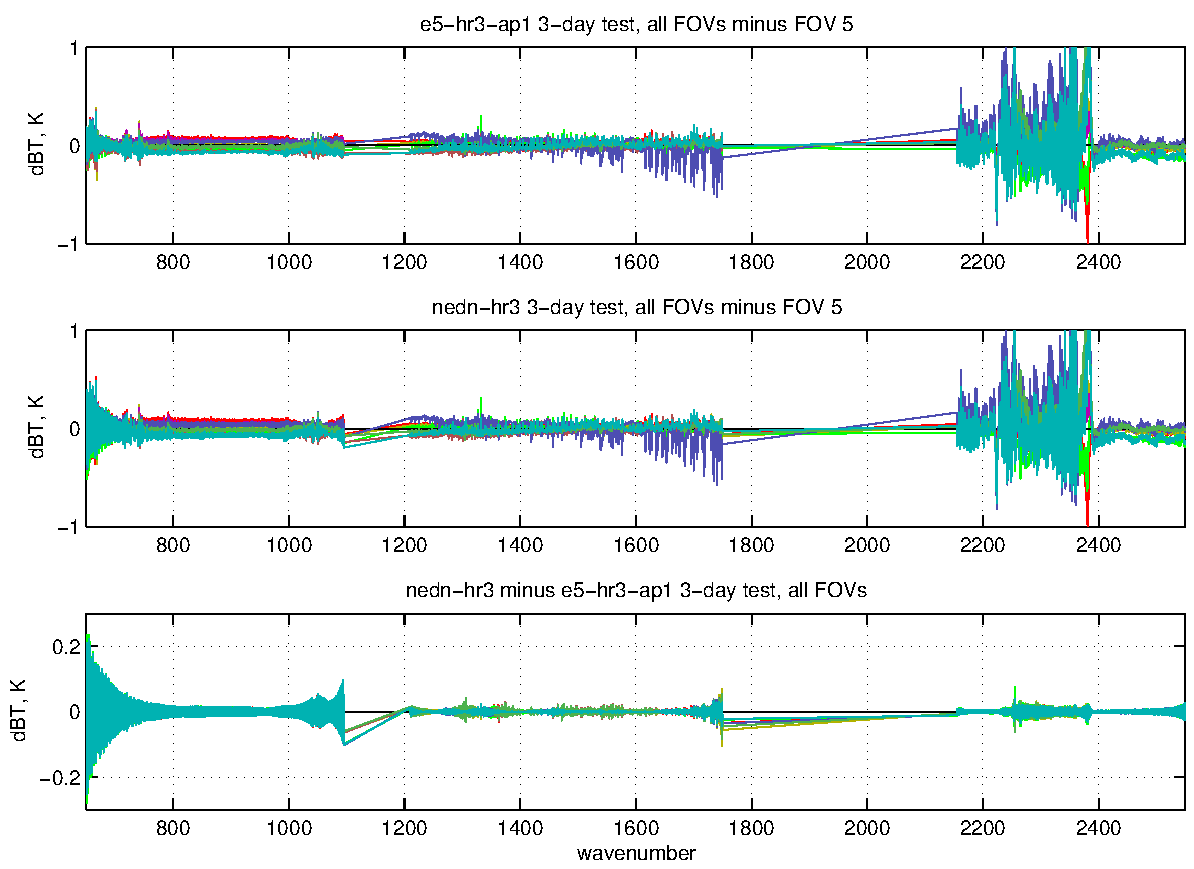
\includegraphics[scale=0.5]{figures/rel_summary.pdf}
\end{center}
\end{frame}

%----------- slide --------------------------------------------------%
\begin{frame}
\frametitle{noaa relative double diffs}
\begin{center}
  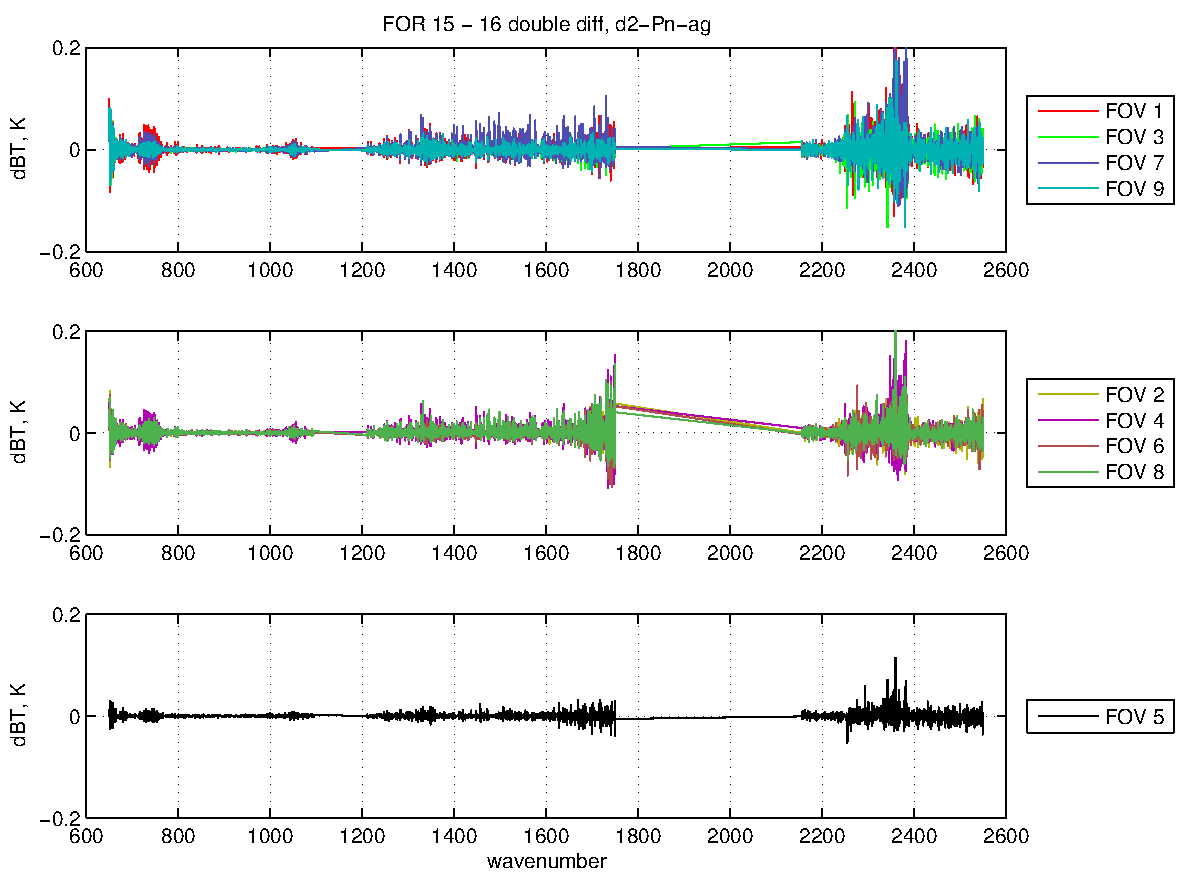
\includegraphics[scale=0.5]{figures/rel_noaa_ddif.pdf}
\end{center}
\end{frame}

%----------- slide --------------------------------------------------%
\begin{frame}
\frametitle{ccast relative double diffs}
\begin{center}
  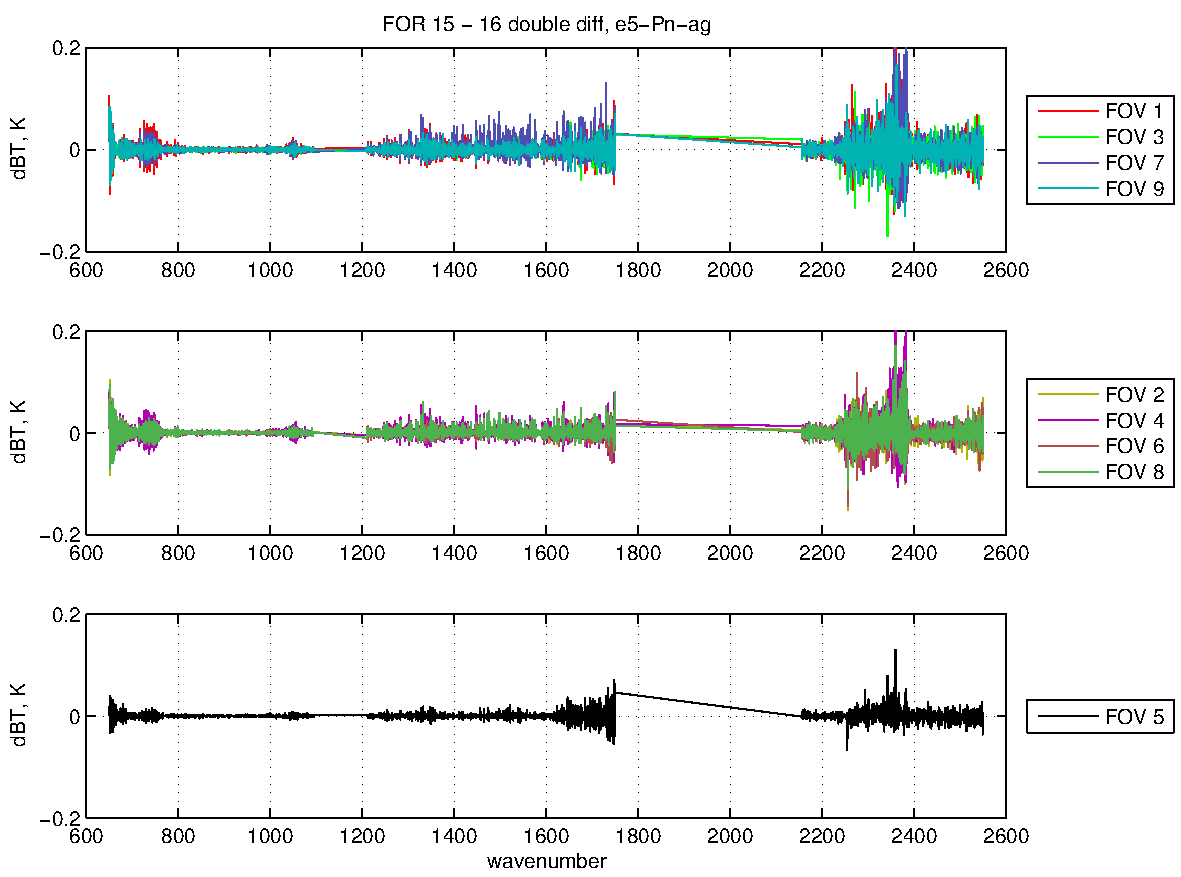
\includegraphics[scale=0.5]{figures/rel_ccast_ddif.pdf}
\end{center}
\end{frame}

%----------- slide --------------------------------------------------%
\begin{frame}
\frametitle{relative test summary}

\begin{itemize}

  \item the overview is the difference from FOV 5 of the means of
    FOR 15 and 16 taken together

  \item the double differences here are \[(\mbox{\small FOR 15} -
    \mbox{\small FOR 16}) - (\mbox{\small apodized FOR 15} -
    \mbox{\small apodized FOR 16})\]

  \item relative test results are generally consistent with the obs
    minus calc tests shown earlier

  \item {\ccast} is worse in the LW and slightly better in the MW
    above around 1600 cm-1.  Some of the LW difference may be due to
    the \fov~5 differences we saw in the obs minus calc tests

  \item the relative double differences are small in comparison with
    other residuals shown here, with {\noaa} a little better overall
    but {\ccast} significantly better for side FOVs in the MW

\end{itemize}

\end{frame}
%----------- slide --------------------------------------------------%
\begin{frame}
\frametitle{conclusions}

\begin{itemize}

  \item we have seen a significant convergence in calibration
    algorithm results and performance

  \item overall the {\noaa} algorithm works slightly better with
    responsivity and {\ccast} better without

  \item remaining differences between the {\ccast} and {\noaa}
    calibration equations are small

  \item {\ccast} flat is slightly worse at the LW end of the LW
    band, and slightly better in the MW above around 1600 cm-1

  \item differences after Hamming apodization are very small

  \item although the {\noaa} algorithm has a few more steps, this
    has no significant effect on runtime

\end{itemize}

\end{frame}
%----------- slide --------------------------------------------------%
\begin{frame}
\frametitle{context for SDR reference truth choices}

\begin{itemize}

  \item {\ccast} flat output close to true sinc \ils

  \item {\ccast} flat RTA simulation requires 3 bandpass filters \\
    (12 parameters)

  \item {\noaa} resp RTA simulation requires full responsivity curves
    (roughly 1700 parameters)


  \item {\noaa} resp radiance climate record may be affected if
    responsivity varies from instrument to instrument or changes for
    a particular instrument

  \item {\cris} flat radiances insensitive to filter characteristic

  \item LLS believe is will be hard to get international community to
    use responsivity in the long time frame!  Debatable

  \item Impact of cal eqn and reference truth choices: Later Talk

\end{itemize}

\end{frame}
%----------- slide --------------------------------------------------%
\begin{frame}
\frametitle{ccast calibration equation}

\[\rES = F \cdot \rIT \cdot f \cdot \SA^{-1}\cdot f \cdot 
         \frac{\ES - \SPmean}{\ITmean - \SPmean} \]

\begin{itemize}
  \item $\rES$ is calibrated earth-scene radiance at the user grid
  \item $F$ is Fourier interpolation from sensor to user grid
  \item $\rIT$ is expected ICT radiance at the sensor grid
  \item $f$ is a raised-cosine bandpass filter with wings at or just
    inside instrument responsivity
  \item $\SA$ is from a periodic sinc ILS wrapping at the sensor
    grid
  \item $\ES$, $\ITmean$ and $\SPmean$ are corrected for
    nonlinearity
  \item $\ITmean$ and $\SPmean$ are averages over 9 scans
\end{itemize}

\end{frame}
%----------- slide --------------------------------------------------%
\end{document}

